\documentclass[a4paper,12pt,twoside]{report}

\usepackage{acronym}
\usepackage{url}
\usepackage{cite}
\usepackage{listings}
\usepackage[pdftex]{graphicx}
\usepackage[hang,small,bf]{caption}
\usepackage{styles/tum}
\usepackage{setspace}
\usepackage[german,english]{babel}
\usepackage{float}
\usepackage{floatflt}
\usepackage{fancyhdr}
\usepackage{color}
\usepackage{booktabs}
\usepackage[pdftex,bookmarks=true,plainpages=false,pdfpagelabels=true]{hyperref}
\usepackage{mdwlist}
\usepackage{enumerate}
\usepackage{paralist}
\usepackage{array}
\usepackage{longtable}
\usepackage{amsmath}
\usepackage{algorithm}
\usepackage[noend]{algpseudocode}
\usepackage{listings}
\usepackage[utf8]{inputenc}
\usepackage[capitalize, noabbrev]{cleveref}
\usepackage{mathtools}
\DeclarePairedDelimiter{\ceil}{\lceil}{\rceil}

% Path for graphics
\graphicspath{{figures/}}

\begin{document}
\setlength{\evensidemargin}{22pt}
\setlength{\oddsidemargin}{22pt}

\def\doctype{Bachelor's Thesis}
\def\faculty{Informatics}
\def\title{Simulation-Based Analysis of Blockchain Architectures}		
\def\titleGer{Simulationsbasierte Analyse von Blockchain Architekturen}
\def\supervisor{Broy, Manfred; Prof. Dr. rer. nat. habil.}
\def\advisor{Marmsoler, Diego; M.Sc.}
\def\author{Leo Eichhorn}
\def\date{15.07.2018}


\hypersetup{pdfborder={0 0 0},
                        pdfauthor={Leo Eichhorn},
                        pdftitle={Simulation-Based Analysis of Blockchain Architectures},
                        }

\lstset{showspaces=false, numbers=left, frame=single, basicstyle=\small}

\pagenumbering{alph}

\thispagestyle{empty}

\vspace{4cm}
\begin{center}
\oTUM{4cm}\\ 
\vspace{5mm}     
\huge DEPARTMENT OF INFORMATICS\\ 
\vspace{0.5cm}
\large TECHNICAL UNIVERSITY OF MUNICH\\
\vspace{1mm}
\end{center}

\vspace{13mm}

\begin{center}
{\Large \doctype\ in \faculty}
\vspace{20mm}

\begin{spacing}{1.5}
{\huge\bf \title}\\%[3ex]
\end{spacing}

\vspace{15mm}
{\LARGE \author}

\vspace{10mm}

\begin{figure}[h!]
\centering
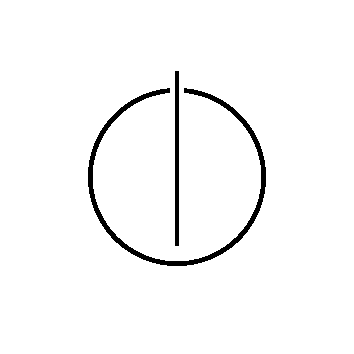
\includegraphics[width=4cm]{InformaticsLogo}
\end{figure}

\end{center}

\thispagestyle{empty}
\pagenumbering{roman}
\vspace{8mm}
\begin{center}
\oTUM{4cm}

\vspace{5mm}     
\huge DEPARTMENT OF INFORMATICS\\ 
\vspace{0.5cm}
\large TECHNICAL UNIVERSITY OF MUNICH\\
\end{center}

\vspace{5mm}

\begin{center}
{\Large \doctype\ in \faculty}
\vspace{8mm}

\begin{spacing}{1.3}
{\LARGE \title}\\
\vspace{8mm}

{\LARGE \titleGer}\\
\vspace{8mm}
\end{spacing}

\begin{tabular}{ll}
\Large Author:     & \Large \author     \\[2mm]
\Large Supervisor: & \Large \supervisor \\[2mm]				
\Large Advisor:	   & \Large \advisor    \\[2mm]
\Large Submission date:       & \Large \date
\end{tabular}

\vspace{1mm}

\begin{figure}[hb!]
\centering
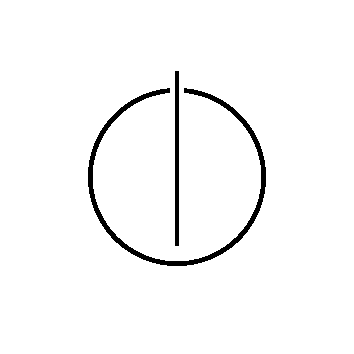
\includegraphics[width=4cm]{InformaticsLogo}
\end{figure}

\end{center}
\newpage
\thispagestyle{empty}
\mbox{}
\clearpage
\thispagestyle{empty}
\vspace*{0.8\textheight}
\noindent
I assure the single handed composition of this bachelor thesis only supported by declared resources,

\vspace{15mm}
\noindent
Munich, \date \hspace{\stretch{1}} \author
\newpage



\newpage
\thispagestyle{empty}
\mbox{}

\chapter*{Acknowledgements}


\pagenumbering{roman}

\selectlanguage{english}
\begin{abstract}

%abstract english

\textit{}

\end{abstract}

\clearpage

\selectlanguage{german}
\begin{abstract}

%abstract german
\textit{}

\end{abstract}

\clearpage

\selectlanguage{english}


\tableofcontents
\clearpage

\clearpage

\begin{acronym}
\acro{RADS}{Resistance of a blockchain architecture against double spend attacks}
\acro{UTXO}{Bitcoin unspent transaction output}
\acro{APSP}{All pairs shortest path problem}
\acro{BTC}{The Bitcoin currency}
\acro{PoW}{Proof of work}
\acro{DSA}{Double-spend attack}
\end{acronym}

\pagenumbering{arabic}

\fancyhead{}
\pagestyle{fancy}
\fancyhead[LE]{\slshape \leftmark}
\fancyhead[RO]{\slshape \rightmark}
\headheight=15pt




%------- chapter 1 -------

\chapter{Introduction}


%------- chapter 2 -------

\chapter{Background}
\section{Blockchain}
A blockchain is a public\footnote{In this thesis, only permissionless blockchains are considered, for permissioned blockchains see for example: \cite{permissioned}}, distributed ledger used to record, identify and verify contracts, transactions or other shared data between multiple parties. The resulting records are stored in a continuously growing list, which is locally maintained and updated by each individual member (\textit{node}) of the protocol. Entries of the list (\textit{blocks}) are cryptographically linked by including a hash of the previous block as a unique identifier in each newly added entry (\autoref{blockchain}). More specifically, altering contents of a block changes its unique identifier, forcing a recalculation of every following block currently in the list, in order to retain integrity of the ledger. If consensus between nodes is reached through proof of work (Section \ref{pow}), performing such an operation consistently requires a substantial amount of computing power, arguably more than 50\% of the total computing power available to the whole Network \cite{nakamoto2008bitcoin}. Newly created blocks are sent to all members to keep local blockchain copies synchronized. By adhering to a distributed consensus protocol, the participating nodes validate potential extensions of their blockchain copy in a peer-to-peer manner, thereby eliminating the need for an intermediary, trusted authority. 

\begin{figure}[ht]
	\centering
  \includegraphics[width=\textwidth]{blockchain.png}
	\caption{Visualization of blocks connected by their hashes}
	\label{blockchain}
\end{figure}
 
\section{Bitcoin} \label{bitcoin}
To gain a better understanding of the blockchain technology and dynamics in a blockchain network, we will provide a short summary of Bitcoin as a concrete example of application. For a more detailed description of the Bitcoin protocol, refer to \cite{nakamoto2008bitcoin,antonopoulos2017mastering,okupski2014bitcoin}.

 Bitcoin is a decentralized digital cryptocurrency created by Satoshi Naka-moto in 2008. In the original Bitcoin paper \cite{nakamoto2008bitcoin}, Nakamoto briefly describes the concepts of the proposed protocol and introduces blockchains as a solution to the apparent double-spending problem. Since Bitcoin is operating entirely on a peer-to-peer basis, a central, monitoring authority, known from services like \textit{Visa} or \textit{Paypal}, does not exist. To still guarantee, that the same transaction cannot be sent multiple times and the sender's capital is sufficient, Nakamoto's blockchain operates as a public ledger and stores each successful transaction, marked with a unique ID. By creating this synchronized and chronological order of transaction events, a sender's liquidity can easily be confirmed by traversing the public blockchain history and calculating the result of all previous transactions. \cite{nakamoto2008bitcoin,bitcoinwiki}

\subsection{Transactions}
Bitcoin wallets and transactions are based on asymmetric cryptography. More specifically, a \textit{wallet} can be described as the collection of a private and a public key \cite{okupski2014bitcoin}. If Alice wants to send a transaction to Bob, she first signs her newly created transaction with the private key of her wallet and specifies the receiver using Bob's public key. By verifying Alice's signature with her public key, Bob is able to proof the authenticity of Alice and the integrity of her transaction. Since Alice's BTC balance isn't represented by a single number, she has to include previous transactions sent to her, as \textit{inputs} to her new transaction to Bob. The values of these input transactions have to sum up to at least the amount of BTC she wants to send to Bob. Since transaction values cannot be divided, Alice can declare her own account as an \textit{output} to her transaction, next to any other receiver, to collect her change. Additional BTCs without corresponding output result in the \textit{transaction fee}, which is used to incentivize miners to include the transaction into their next block. The fee is claimed by the first node incorporating the transaction into the blockchain. The process of using existing transactions as inputs for new transactions leads to the strict distinction between \textit{spent} and \textit{unspent} transaction output (UTXO). The sum of UTXOs therefore determines the current balance of a Bitcoin account.

In \autoref{fig1}, Alice creates a new transaction and uses two of her accounts to send 2 BTC to Bob. She specifies the UTXOs she would like to use as inputs and leaves 0.02 BTC as a transaction fee. In transaction 817, Alice and Bob each send 0.05 BTC to Charlie, by using the UTXOs of the previous transaction. \cite{DSAwithTime}
\begin{figure}[ht]
	\centering
  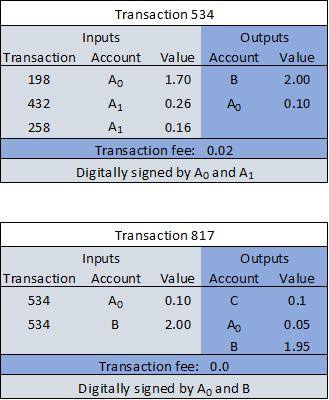
\includegraphics[scale=0.7]{TransactionExample.png}
	\caption{Example of two BTC transactions (simplified) \cite{DSAwithTime}}
	\label{fig1}
\end{figure}

Alice sends her new transaction to each of her Bitcoin peers, where it is added to a temporary pool of unverified transactions. Before it is further propagated down the network, Alice's peers verify the new transaction, which includes validation of the UTXOs referenced as inputs and the participating members. After verification, the transaction is added to a pool of valid transactions (\textit{memory pool}) and is sent to the next peers. \cite{antonopoulos2017mastering}

\subsection{Blocks}
For transactions to be confirmed and added to the ledger of valid transactions in the blockchain, they first have to be included in a block and the \textit{proof of work} (Section \ref{pow}) has to be calculated. Potential transactions for the next block are selected from each node's memory pool, whereas transactions with higher fees are prioritized. The main parts of a Bitcoin block are depicted in \autoref{fig2} and consist of a block \textit{header} and \textit{body}. The block header includes the current Version of the Bitcoin protocol, a timestamp of the block creation, a hash\footnote{More specifically the root of a merkle tree built from all transaction \cite{okupski2014bitcoin}} of this block's body and a double-SHA256 hash of the previous block's header. When a new block is created, the previous block field is set to the hash of the most recent block currently on the blockchain. By inserting this hash into the new block, the two blocks can be interlinked and the blockchain extended. This leads to a continuous backwards connection of all blocks up to the \textit{genesis block}. The genesis block is the first block created by Satoshi Nakamoto in 2009 and is statically encoded in each Bitcoin client's software \cite{antonopoulos2017mastering}. Two additional fields, the current mining difficulty and a nonce are used to calculate the proof of work. The block body contains all transactions added to this block, including a \textit{coinbase transaction} which will be redeemed by the first node successfully calculating this block's proof of work. The coinbase transaction contains the sum of all transaction fees included in the block and the current \textit{block reward}. Giving rewards for mining a block is Bitcoin's way of releasing new BTC to the network and providing an incentive for miners to contribute their resources to the system. \cite{okupski2014bitcoin,antonopoulos2017mastering}
\begin{figure}[ht]
	\centering
  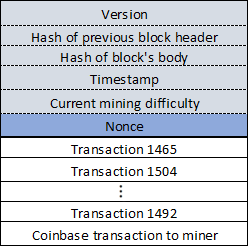
\includegraphics[scale=0.7]{BlockExample.png}
	\caption{Example of a Bitcoin block header (blue) and body (white) \cite{DSAwithTime,okupski2014bitcoin}}
	\label{fig2}
\end{figure}

\subsection{Proof of Work} \label{pow}
To add a block to the blockchain, a valid proof of work has to be calculated, which is also known as \textit{mining} a block. To mine a block, the node (\textit{miner}) repeatedly calculates the double-SHA256 hash of the block's header, while updating the nonce value. The proof of work is treated as valid, once the calculated hash starts with a specific number of zero digits, which is called the \textit{mining difficulty}. Since SHA256 is considered to be irreversible, brute-forcing the nonce value to generate a new hash each time is the most efficient way of mining a block. The number of required zeros is specified in the block header and increases over time. This is done in order to keep the network from mining more than the intended average of 6 blocks per hour, while hardware and computational power increases. The validity of a block's proof of work can easily be verified by hashing its header once again and testing the result against the target mining difficulty. Since a single node rarely has enough computational power to calculate a valid proof of work in a reasonable time, miners often collude in \textit{mining pools} by sharing any generated block reward, based on the amount of hashes calculated by each node. \cite{antonopoulos2017mastering,okupski2014bitcoin}

Since every change in a block's header results in a different hash, calculating the proof of work ensures, that once a block has been added to the blockchain, the block and its transactions can only be modified, by recalculating the proof. In fact, each block that was added after the modified block would have to be recalculated as well, since each block contains the hash of its previous block. By changing the hash of a block, the header of the following block would also have to be changed, thereby invalidating its proof of work. \cite{nakamoto2008bitcoin}

\subsection{Peer-to-peer Network}
After the valid proof of work is computed, the successfully mined block is appended to the local blockchain copy and sent to the miner's peers. Before adding the new block to their own copy of the blockchain and further propagating it in the network, the peers ensure that there exists a hash of any block in their blockchain that corresponds to the hash specified in the new block's header. Blocks without a known parent are called \textit{orphaned blocks}\footnote{In literature oprhaned blocks are sometimes used as a term for valid blocks, that are no longer part of the main chain, after a fork. According to \cite{staleblocks}, we will refer to these blocks as stale blocks instead.} and are temporarily stored since the missing parent block might be transmitted in the future. If the new block does reference an existing block in the blockchain, contains only valid transactions and satisfies the current mining difficulty with its proof of work, the block is appended to the correct parent in the local blockchain and sent to the next peers. 

Because Bitcoin operates on a peer-to-peer basis, latencies in the network are unavoidable. According to \cite{infoprop}, the mean time until a
node receives a new block is 12.6 seconds, while approximately 5\% of nodes still have not received the block after 40 seconds. Since a new Bitcoin block is created \textit{on average} every 10 minutes, it is possible that two miners find solutions to two different blocks at roughly the same time, thereby creating a \textit{fork} of the blockchain (\autoref{blockchainfork}). This results in a situation, in which the local blockchain copies of some peers are no longer synchronized. To resolve this conflict and to regain consensus between nodes, a simple rule is employed. According to the bitcoin protocol, nodes are always mining on the blockchain containing the most proof of work, which more or less corresponds to the fork with the highest number of blocks. If two forks containing the same amount of blocks are available, miners are encouraged to work on the fork they received first. This ensures, that even if there are two versions of the blockchain with the same length, nodes will keep mining on any of the two forks until a new block is found. By appending the new block to one of the forks, the contained proof of work increases and miners working on the other fork will switch to the longer chain, thereby resolving the race. Subsequently, the blocks of the losing fork are invalidated and their transactions are released back into the network. These blocks are known as \textit{stale} blocks. \cite{okupski2014bitcoin}
\begin{figure}[ht]
	\centering
  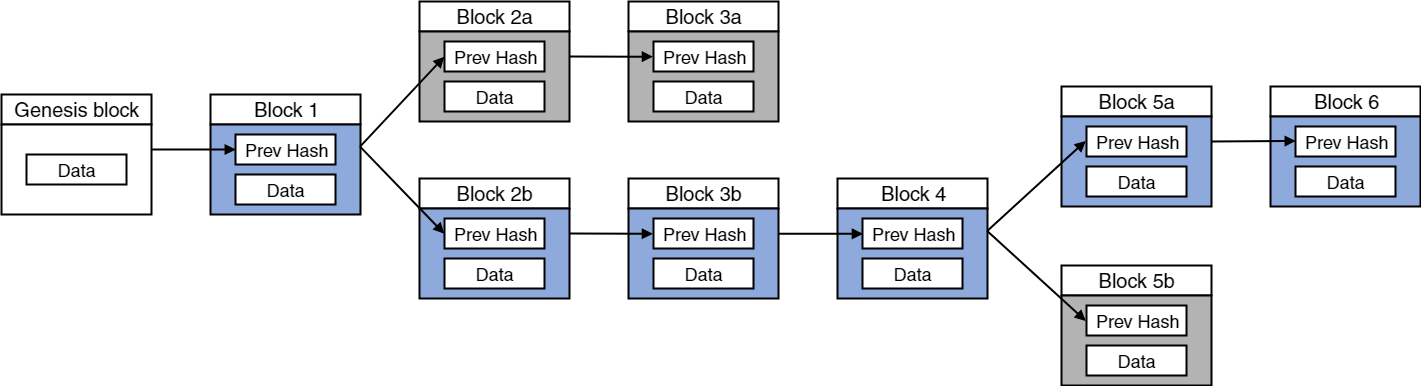
\includegraphics[width=\textwidth]{BlockchainFork.png}
	\caption{Blockchain with two stale branches (gray) forking from the valid chain (blue) }
	\label{blockchainfork}
\end{figure}

To avoid problems with invalidated blocks and transactions due to these kinds of races and attacks similar to the one presented in Section \ref{pow}, Bitcoin introduced the concept of \textit{confirmations}. If Alice's transaction is validated and successfully mined into a block on the blockchain, it receives \textit{one} confirmation. For each additional block mined onto the chain, after the block containing Alice's transaction, it receives another confirmation. Consequently, the number of confirmations corresponds to the number of blocks that would have to turn stale, or have to be recalculated, in order to invalidate Alice's transaction. Over the history of Bitcoin, the number of six confirmations has been widely accepted as a common standard. However, since waiting for six confirmations means waiting approximately one hour for the transaction to be valid, a lot of services operate on only a few, or even no confirmations, which can lead to several problems further described by \cite{premining1}. In comparison, coinbase transactions to reward the miner of a new block, are considered to be valid only after they have been confirmed by a total of 100 mined blocks. \cite{antonopoulos2017mastering}

\section{Double-spend Attacks} \label{dsa}
In \cite{nakamoto2008bitcoin}, Nakamoto claims to have solved the double-spending problem with his proposal of the Bitcoin protocol. Nevertheless, attacks on Nakamoto's blockchain architecture to generate double-spending transactions are still possible and can be described as a series of events:
\begin{enumerate}
\item An attacker \textit{A} would like to receive a service or product from a target merchant \textit{M}.
\item \textit{A} generates two transactions:
\begin{itemize}
\item \textbf{T\textsubscript{M}}, to pay the merchant.
\item \textbf{T\textsubscript{A}}, to send the money back to \textit{A}. Created by specifying \textit{A} as output while using the same inputs of \textbf{T\textsubscript{M}}.
\end{itemize}
\item \textit{A} broadcasts \textbf{T\textsubscript{M}} and starts mining on a secret branch extending the most recent block. A includes \textbf{T\textsubscript{A}} into the first block of the new branch.
\item Once \textbf{T\textsubscript{M}} is confirmed by the remaining network, \textit{M} delivers the product or service to \textit{A}.
\item If necessary, \textit{A} keeps mining on the secret branch containing \textbf{T\textsubscript{A}} until it is longer than the honest branch.
\item \textit{A} releases her now longer branch, thereby invalidating each block of the honest branch, including the block containing \textbf{T\textsubscript{M}}.
\item All nodes start mining on the longer branch. Since \textbf{T\textsubscript{A}} is now part of the valid blockchain, \textit{A} gets to keep M's payment and the delivered product.
\end{enumerate}
For this attack to succeed, \textit{A} needs to mine blocks onto the secret blockchain branch faster than the remaining network confirming the transaction to the merchant. According to \cite{nakamoto2008bitcoin}, consistently winning this race, requires the majority of hashingpower in the network. Nevertheless, this attack is always possible, even with less hashing power, at the cost of an increasing amount of failed attempts. \cite{HBDSA,DSAwithTime}


%------- chapter 3 -------

\chapter{Related Work}
\section{Hashrate-based Models for Double-Spend Attacks}
Potential attacks on blockchains, especially the Bitcoin protocol, have been conceptualized since the release of Nakamoto's original Bitcoin paper \cite{nakamoto2008bitcoin}. In chapter 11 of his proposal, Nakamoto formulates the first mathematical model to calculate the theoretical probability of successful double-spend attacks on his protocol. This model has since been improved and adapted several times, while similar, independent models have been formulated as well \cite{HBDSA,DSAwithTime,NakamotoDSACorrection,NakamotoExplMCSim}. Similar to \cite{DSAwithTime}, we will call the collection of these approaches \textit{hashrate-based} attack models. The central premise of a hashrate-based model is splitting the total computing power available to the network (hashrate \textit{H}), into two parts. To achieve this, \cite{HBDSA} defines \textit{pH} as the hashrate controlled by honest nodes adhering to the protocol, while \textit{qH} is used by malicious nodes trying to attack the blockchain. Since also
\begin{equation}
p + q = 1
\end{equation}
it can easily be seen that \textit{p} and \textit{q} are precisely the probabilities of the next block being mined by either the honest or the attacking part of the network. Using an adaptation of the Gambler's Ruin problem \cite{gamblersruin}, Nakamoto and \cite{HBDSA} are now calculating the probability \textit{Q\textsubscript{z}} of an attacker successfully catching up with their fork of the blockchain, asuming they are at a total deficit of \textit{z} blocks compared to the honest nodes. The success of a potential double-spend attack against a merchant waiting for \textit{n} confirmations can now be formulated as the probability of \textit{Q\textsubscript{z}}, after \textit{n} blocks have been mined by the honest network. While \cite{nakamoto2008bitcoin} is using a poisson distribution in his formula, \cite{HBDSA} is achieving similar results with a negative binomial distribution. Combined with \cite{NakamotoDSACorrection}, the author of \cite{HBDSA} is also pointing out and correcting an of-by-one error introduced by Nakamoto, who is only calculating the probability of an attacker \textit{catching up} with his fraudulent blockchain fork, while for the double spend attack to be successful, the length of the honest chain has to be \textit{surpassed}. \cite{DSAwithTime} presents two similar approaches but considers partial advancement towards block creation as well. The author's first model extends the hashrate-based model formulated by \cite{HBDSA} and includes an additional parameter, indicating the time an attacker has already spent mining on blocks. The second model is fundamentally based on the time differences at which honest and attacking nodes have mined their last block, but is also relying on hashrates as a measure of computational power.
It is interesting to note that all of the before mentioned models produce similar results, despite the differences in their calculations. Therefore it is less surprising, that the authors seem to agree on their general conclusions as well. Those can be summarized as follows:
\begin{itemize}
\item If an attacker controls the majority of computational power in the network, double-spend attacks will always succeed.
\item Probabilities for successful double-spend attacks decrease exponentially with an increasing number of confirmations.
\item Probabilities for successful double-spend attacks increase exponentially with an increasing amount of hashingpower controlled by the attacker.
\item Although double-spend attacks at the standard of six confirmations are considered to be unlikely, there is nothing special about the number six.
\item Double-spend attacks are always possible, regardless of the number of confirmations and amount of computational power controlled by the attacker.
\end{itemize}
\section{Simulations}
An important remark can be seen in the fact that none of the before mentioned hashrate-based models have been confirmed or supported by experimental data or tests in an exhaustive and realistic way. Instead, the validity of these models relies mostly on mathematical proofs and expertise, or the comparison with other, similar models. Nevertheless, one exception can be made with \cite{NakamotoExplMCSim}. After presenting a detailed explanation of Nakamoto's model for double-spends, the author validates the mathematical approach by performing a Monte Carlo simulation \cite{montecarlo} with different sets of input. In the light of this, the author identifies an error of the model, which is linked to its use of the poisson distribution. In spite of this success, the Monte Carlo simulation is missing parameters of a real blockchain protocol and ``does not actually
mine coin, it simply flips some coins to see whether each miner wins a block as simulated'' \cite{NakamotoExplMCSim}. A more realistic simulation of a different attack on Bitcoin blockchains, the selfish-mine attack, is presented by \cite{mwalemodel} and \cite{selfishmine2}. In these two models of the Bitcoin protocol, random (\textit{x}, \textit{y})-coordinates of a two dimensional plane are assigned to each node, in order to create a simple network topology. By simulating the latency between two nodes as proportional to their euclidean distance in the plane, both authors successfully model block propagation times of a real network. During the simulation, new blocks are again generated as instances of a poisson process with an average rate of ten minutes. 
\section{Other Attacks}
Next to double-spend atttacks, a wide variety of different attacks against blockchains and the Bitcoin protocol have been conceptualized. The already mentioned \textit{selfish-mine attack}, or \textit{block-discarding attack}, focuses on invalidating the honest miners' work, by selectively publishing premined blocks to the network \cite{mwalemodel,selfishmine1,selfishmine2,lessThanHalfDraft}. According to \cite{lessThanHalfDraft} and \cite{selfishmine1} this attack can succeed with only a fraction of 25\% total hashing power controlled by the attacker. The \textit{whale attack} presented by \cite{whaleattack} aims to increase an attacker's chances of successful double-spends by publishing transactions with large mining fees, to incentivize honest miners to build on a fraudulent blockchain fork. \cite{premining1} and \cite{premining2} further capitalize on the \textit{premining} strategy of secretly mining blocks ahead of the honest blockchain, while also including a reversed transaction to the target. Once the attacker has gained a comfortable lead, the original transaction to the target merchant is released. Now the lead of the attackers' fork only has to be maintained until the transaction has been confirmed, in order to perform a double-spend. The authors demonstrate how this attack can be used to increase the probability of double-spend attacks, when timing of the transaction used as bait is not important.
\section{Contribution}
It can clearly be observed, that despite the impressive amount of work being done towards the formalization of theoretical attack models against blockchains and especially double-spends attacks, barely anything has been validated by empirical evidence or data. Instead, correctness of the proposed models is achieved by mathematical proofs, while arguably important factors of blockchain dynamics are disregarded or hidden behind intangible parameters like the ``hashrate''. In this thesis we will therefore counter this trend and design a \textit{java} framework to model simulations of blockchain architectures. This framework will subsequently be used to implement an exemplary simulator for double-spend attacks. The goal is to increase the understanding of factors affecting the resistance of blockchain architectures against double-spend attacks and to improve an architect's predictions based on results generated by the model. This will be achieved by conducting experiments based on real world inspired parameters of a blockchain protocol using our simulator. These parameters include specifically:
\begin{itemize}
\item The number of attacking and trusted nodes
\item The difficulty of mining a new block
\item The number of confirmations used by the target
\item Topology and density of the attacking and defending network
\item Latency in the attacking and defending network
\item Latency of the connection between attacking and defending network
\end{itemize}
Using these parameters and the simulator framework, we will then propose our own mathematical model for double-spend attacks, based on data generated by several experiments and tests.
%------- chapter 4 -------

\chapter{The Blockchain Simulator}

\section{Simulation Framework}
To simplify future implementation and simulation of other attacks on block-chains, the core part of our simulator represents an extensible, abstracted framework for general blockchain architectures. By subclassing the existing elements of the framework, the simulator's functionality can be extended and customized, in order to model specific blockchain dynamics. Compared to the example blockchain protocol presented in Section \ref{bitcoin}, a few adaptations have been made:
\begin{itemize}
\item Every node of the network is a miner.
\item Each miner is represented by a single program thread.
\item Instead of hashing a block and updating nonce values, mining a block consists of repeatedly generating random numbers until a number lower than the target difficulty is found.
\item The framework does not include generation and transmission of transactions, since the data contained inside the blocks is not relevant to our investigations.
\item Instead of sending single blocks, miners propagate whole copies of their local blockchains along the network.
\item Nodes start mining on a received blockchain if it is longer than the blockchain currently being mined on.
\item Latency time between two peers is constant and symmetric.
\end{itemize}
\subsection{Classes}
\begin{figure}[ht]
	\centering
  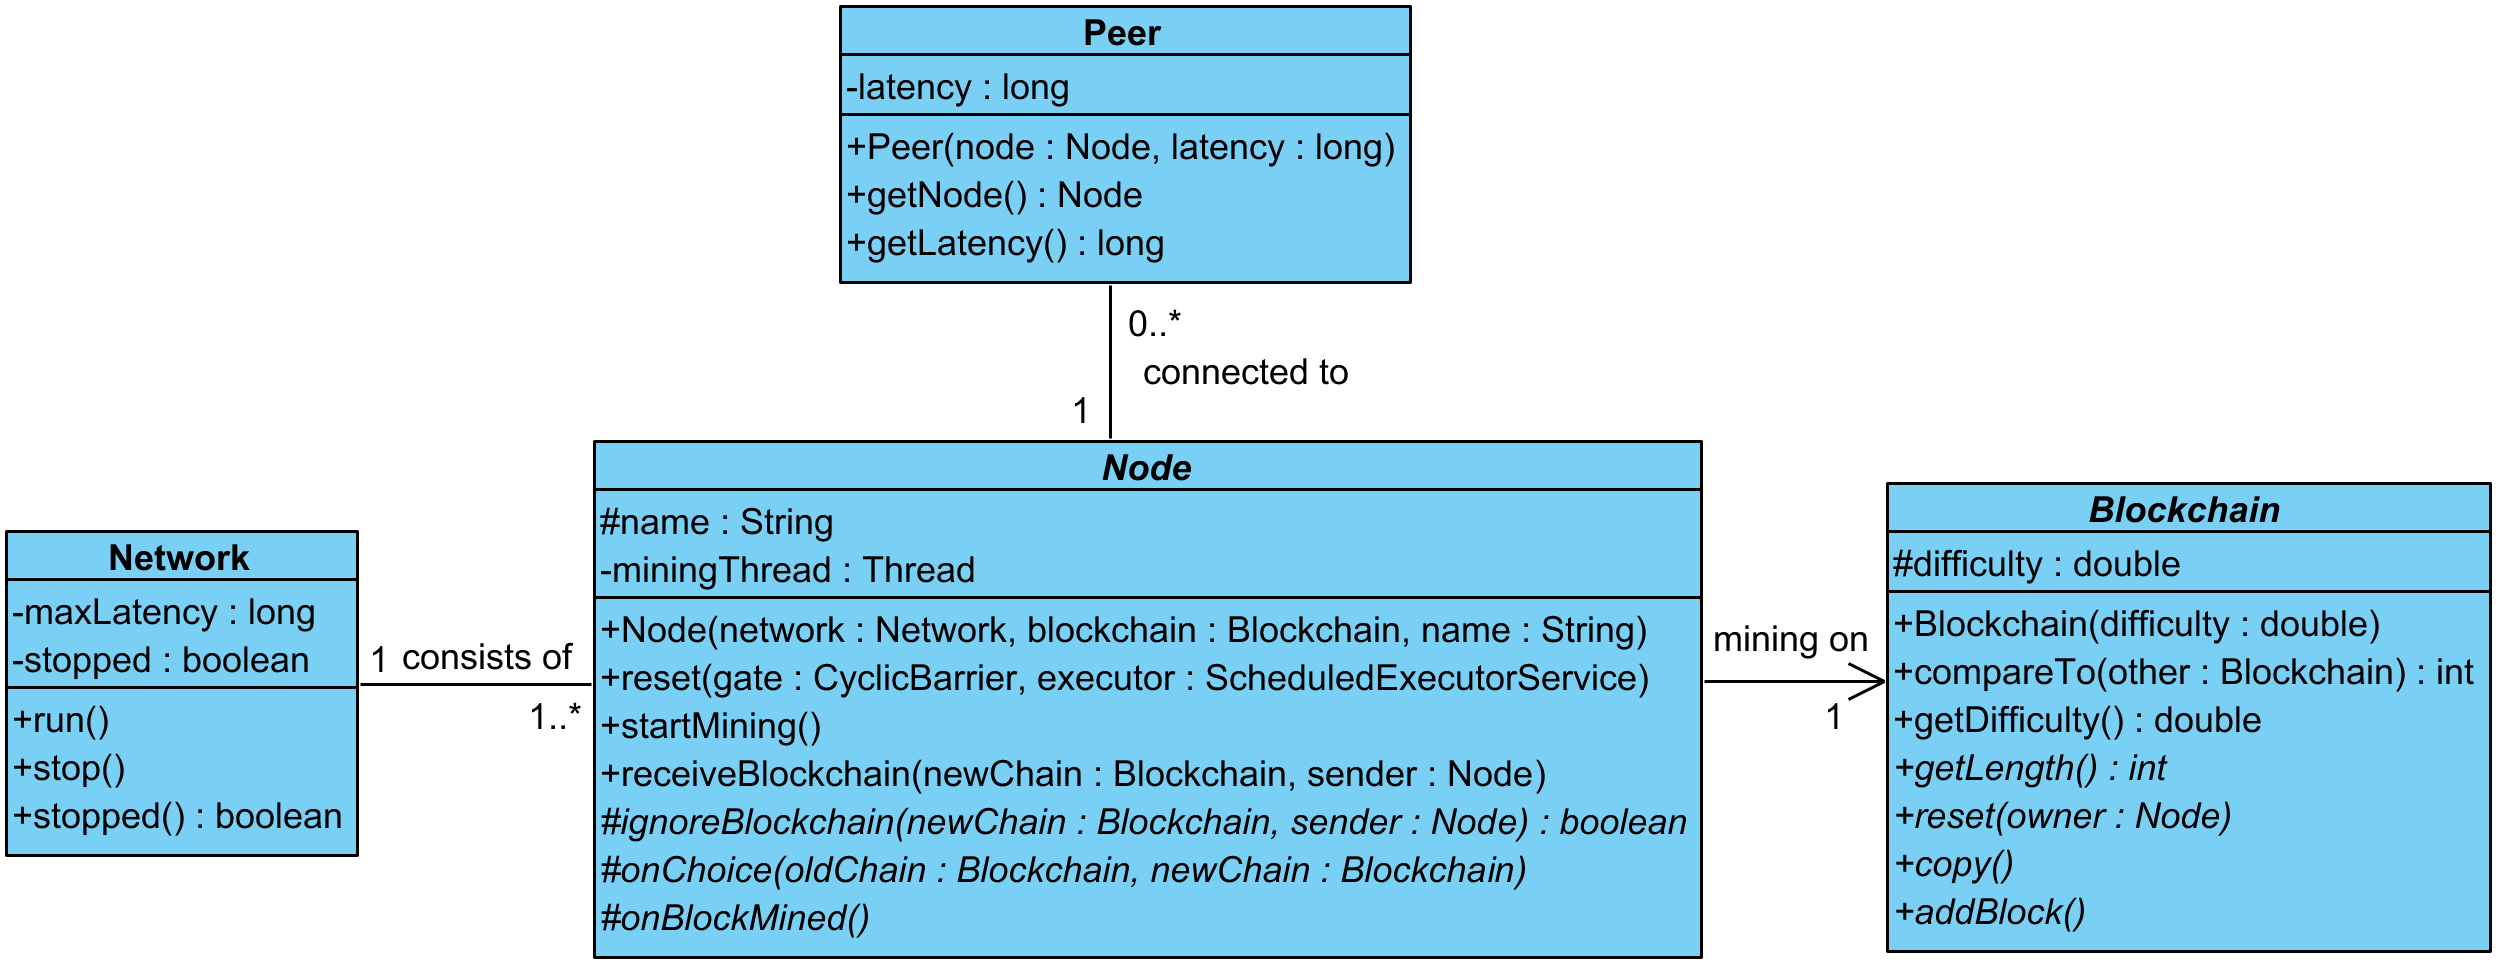
\includegraphics[width=\textwidth]{Framework.png}
	\caption{Class diagram of the blockchain simulation framework}
	\label{framework}
\end{figure}

\subsubsection{Node}
The node represents a basic implementation of a honest miner adhering to our blockchain protocol. Each node contains a reference to every other node in the network using the peer class. Once a new block is mined, it is added to the local blockchain and, after the corresponding latency times, a copy of the blockchain is sent to all peers. The node will only start mining on a newly received blockchain if it is longer than the local blockchain copy. To simplify execution of multiple simulation runs, each node can be reset to their initial state. To allow simulation of nodes diverging from the standard protocol, the class contains three abstract methods which can be implemented to alter the behavior of the node. 

\subsubsection{Peer}
To represent the connection to a node in the network, the peer is implemented as a simple data class, containing the latency time in milliseconds needed to reach the referenced node.

\subsubsection{Blockchain}
In order to allow concrete implementations of different blockchain models, the blockchain class only provides the abstracted interface required by nodes. An implementation of the blockchain class therefore contains routines for adding a block and returning the length of the blockchain. Since nodes propagate whole copies of the blockchain instead of single blocks, a method of copying the blockchain has to be implemented as well.

\subsubsection{Network}
The network acts as a central controller of the blockchain framework. It maintains references to all nodes in the network and provides simple routines for starting and stopping the mining processes of all nodes in a synchronized manner. Once the network is started, the calling thread of \textit{run()} is blocked until the execution of all nodes is completed. The nodes terminate their mining threads after the network is stopped, which is ideally done as a consequence of some end condition reached by the simulation.


\subsection{Creating the Peer-to-peer Network} \label{peerstratsection}
Apart from simulating blockchains and miners, the simulator framework requires additional functionality to model different forms of peer-to-peer networks. The general task is to create a connected graph of all nodes, whereas edges and edge weights represent the latency times between two nodes. Using the strategy pattern\cite{strategy}, the simulator framework provides implementations of five different ways of modeling the network (\autoref{peerstrategy}), while additional strategies can easily be added in the future. The different peer strategies are used by instantiating the specific strategy and calling the \textit{connectPeers()} method with a list of all nodes in the network. The strategy will then populate the peer lists of each node accordingly. In the following an overview of all available strategies will be provided.
\begin{figure}[ht]
	\centering
  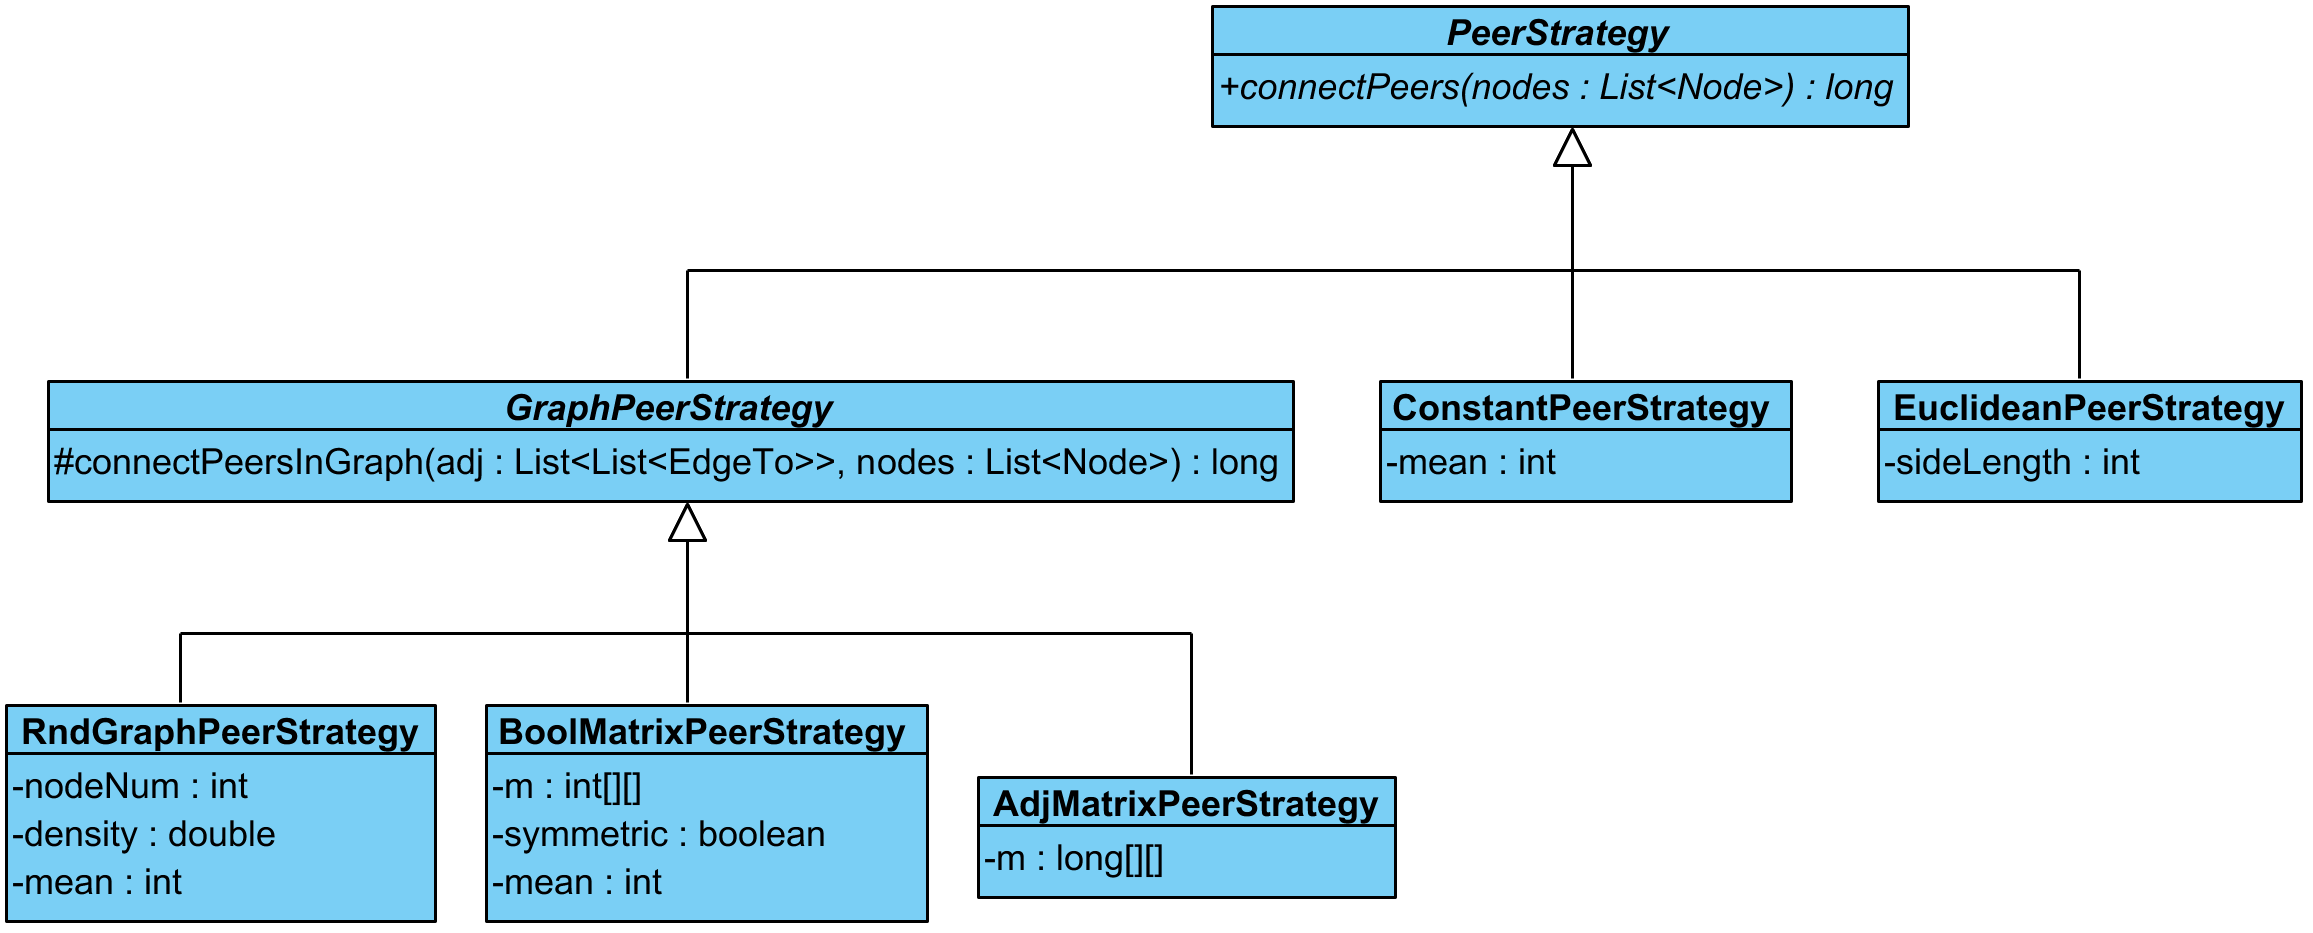
\includegraphics[width=\textwidth]{PeerStrategy.png}
	\caption{Class diagram of the different strategies available to connect nodes in the peer-to-peer network}
	\label{peerstrategy}
\end{figure}
\subsubsection{ConstantPeerStrategy}
All nodes in the network are connected by symmetric latencies $l$, sampled from a normal distribution with constant mean $m$. The standard deviation is calculated using a constant deviation factor $c$ and the mean. Unless otherwise specified, $c$ equals $0.1$.
\begin{equation}\label{distribution} 
l\in L\sim cm\mathcal{N}(0,1)+m = \mathcal{N}(m,c^{2}m^{2})
\end{equation}
\subsubsection{EuclideanPeerStrategy}
Similar to the models presented by \cite{mwalemodel} and \cite{selfishmine2}, all Nodes are assigned random coordinates $(x,y)$ in a two dimensional, quadratic plane. The latency between two Nodes $p$ and $q$ is sampled from a normal distribution whose mean $m$ is equal to the nodes' euclidean distance as defined by Equation \ref{distribution}.
\begin{equation}\label{euclid}
m = \sqrt{(p_{x}-q_{x})^{2}+(p_{y}-q_{y})^{2}}
\end{equation}
By setting the strategy's \textit{side length} parameter, the area of the square can be defined. Creating a bigger plane consequently leads to overall higher latencies in the network.
\subsubsection{AdjMatrixPeerStrategy}
This strategy creates a graph of nodes according to a given adjacency matrix. Latencies between two nodes are represented by the matrix entries, whose indices refer to the corresponding nodes in the provided list. Negative entries indicate that there is no connection between two nodes, whereas a value of zero leads to a connection without latency. Choosing the entry values allows simulation of typical network topologies like stars and rings. After creating the graph, Dijkstra's shortest path algorithm\cite{dijkstra} is used to solve the all pairs shortest path (APSP) problem. With the resulting distance matrix, all peers of each node can be initialized.
\subsubsection{BoolMatrixPeerStrategy}
Similar to the previous strategy, a graph is created as specified by the given adjacency matrix. This time, positive entries of the matrix only indicate existence of a connection between two nodes, whereas negative and zero values lead to no connection in the graph. The latencies are instead sampled from a normal distribution with constant mean as defined by formula \ref{distribution}.
\subsubsection{RndGraphPeerStrategy} \label{rndgraphstrategy}
This strategy generates a pseudo-random graph with a given number of nodes and edges. To avoid the intangible scale of a parameter defining the number of edges, the graph density $d$ is used instead. Since the generated graph has to be connected, the number of edges $e$ is calculated from $d$ and the number of nodes $n$ as shown in equation \ref{dens}. 
\begin{equation}\label{dens}
e = max \left( d\frac{n\left( n-1\right) }{2}, n-1 \right), d\in [0,1]
\end{equation}
It is important to note, that the created graph is not entirely random, as Algorithm \ref{rndgraph} introduces a bias by always selecting a visited node for one end of a new edge. Since for each iteration, only visited nodes are considered, earlier nodes are more likely to receive a higher degree.\cite{stackoverflow} 

Edge weights of the graph corresponding to the latency between two nodes are sampled according to formula \ref{distribution}. The distances between all nodes used to initialize each node's peers are again calculated by Dijkstra's APSP algorithm. 
\begin{algorithm}
\caption{Creates a pseudo-random, undirected, connected graph with the given number of nodes and edges}\label{rndgraph}
\begin{algorithmic}[1]
\Procedure{RndGraph}{nodes, edges}
\State $\textit{G} \gets \textit{(V, E)}$
\State $i \gets 0$
\State $V \cup \{i \}$
\While {$++i < \textit{nodes}$}
\State $u \gets \textit{rndElement(V)}$
\State $V \cup \{i \}$
\State $E \cup \{(i,u),(u,i) \}$
\EndWhile
\State $e \gets edges - (nodes-1)$
\While {$e-- > 0$}
\State $E' \gets \textit{missingEdges(G)}$
\State $(x,y) \gets \textit{rndElement(E')}$
\State $E \cup \{(x,y),(y,x) \}$
\EndWhile
\State \Return $G$
\EndProcedure
\end{algorithmic}
\end{algorithm}

\section{Double-Spend Simulation}
In order to simulate double-spend attacks, we split the miners modeled by the blockchain framework into two parts and create two subclasses of the framework's node implementation. The newly created trusted nodes adhere to our simplified blockchain protocol and keep mining on the longest branch they are currently aware of. The attacking nodes, trying to generate a double-spending transaction, are mining blocks to extend their secret branch. Both groups of nodes are combined into an attacking and trusted network, by using two instances of the peer strategies presented in Section \ref{peerstratsection}. Unless otherwise specified, the double-spend simulator uses two RndGraphPeerStrategies and recreates the resulting graphs randomly before every new simulation run. Initially, consent of all nodes is on a blockchain of size \textit{0}, containing the most recent block before \textbf{T\textsubscript{M}} and \textbf{T\textsubscript{A}} (Section \ref{dsa}) are published. It is assumed that both transactions are mined into the first block of their corresponding networks. After \textbf{T\textsubscript{M}} is confirmed with the simulated number of confirmations, the merchant's product is assumed to be sent. The attackers then start publishing their branch including \textbf{T\textsubscript{A}}, to convince the trusted network of their alternate transaction history not containing \textbf{T\textsubscript{M}}. The double-spend is considered to be successful, once all trusted nodes are mining on the blockchain containing \textbf{T\textsubscript{A}}.
\subsection{Classes}
\begin{figure}[ht]
	\centering
  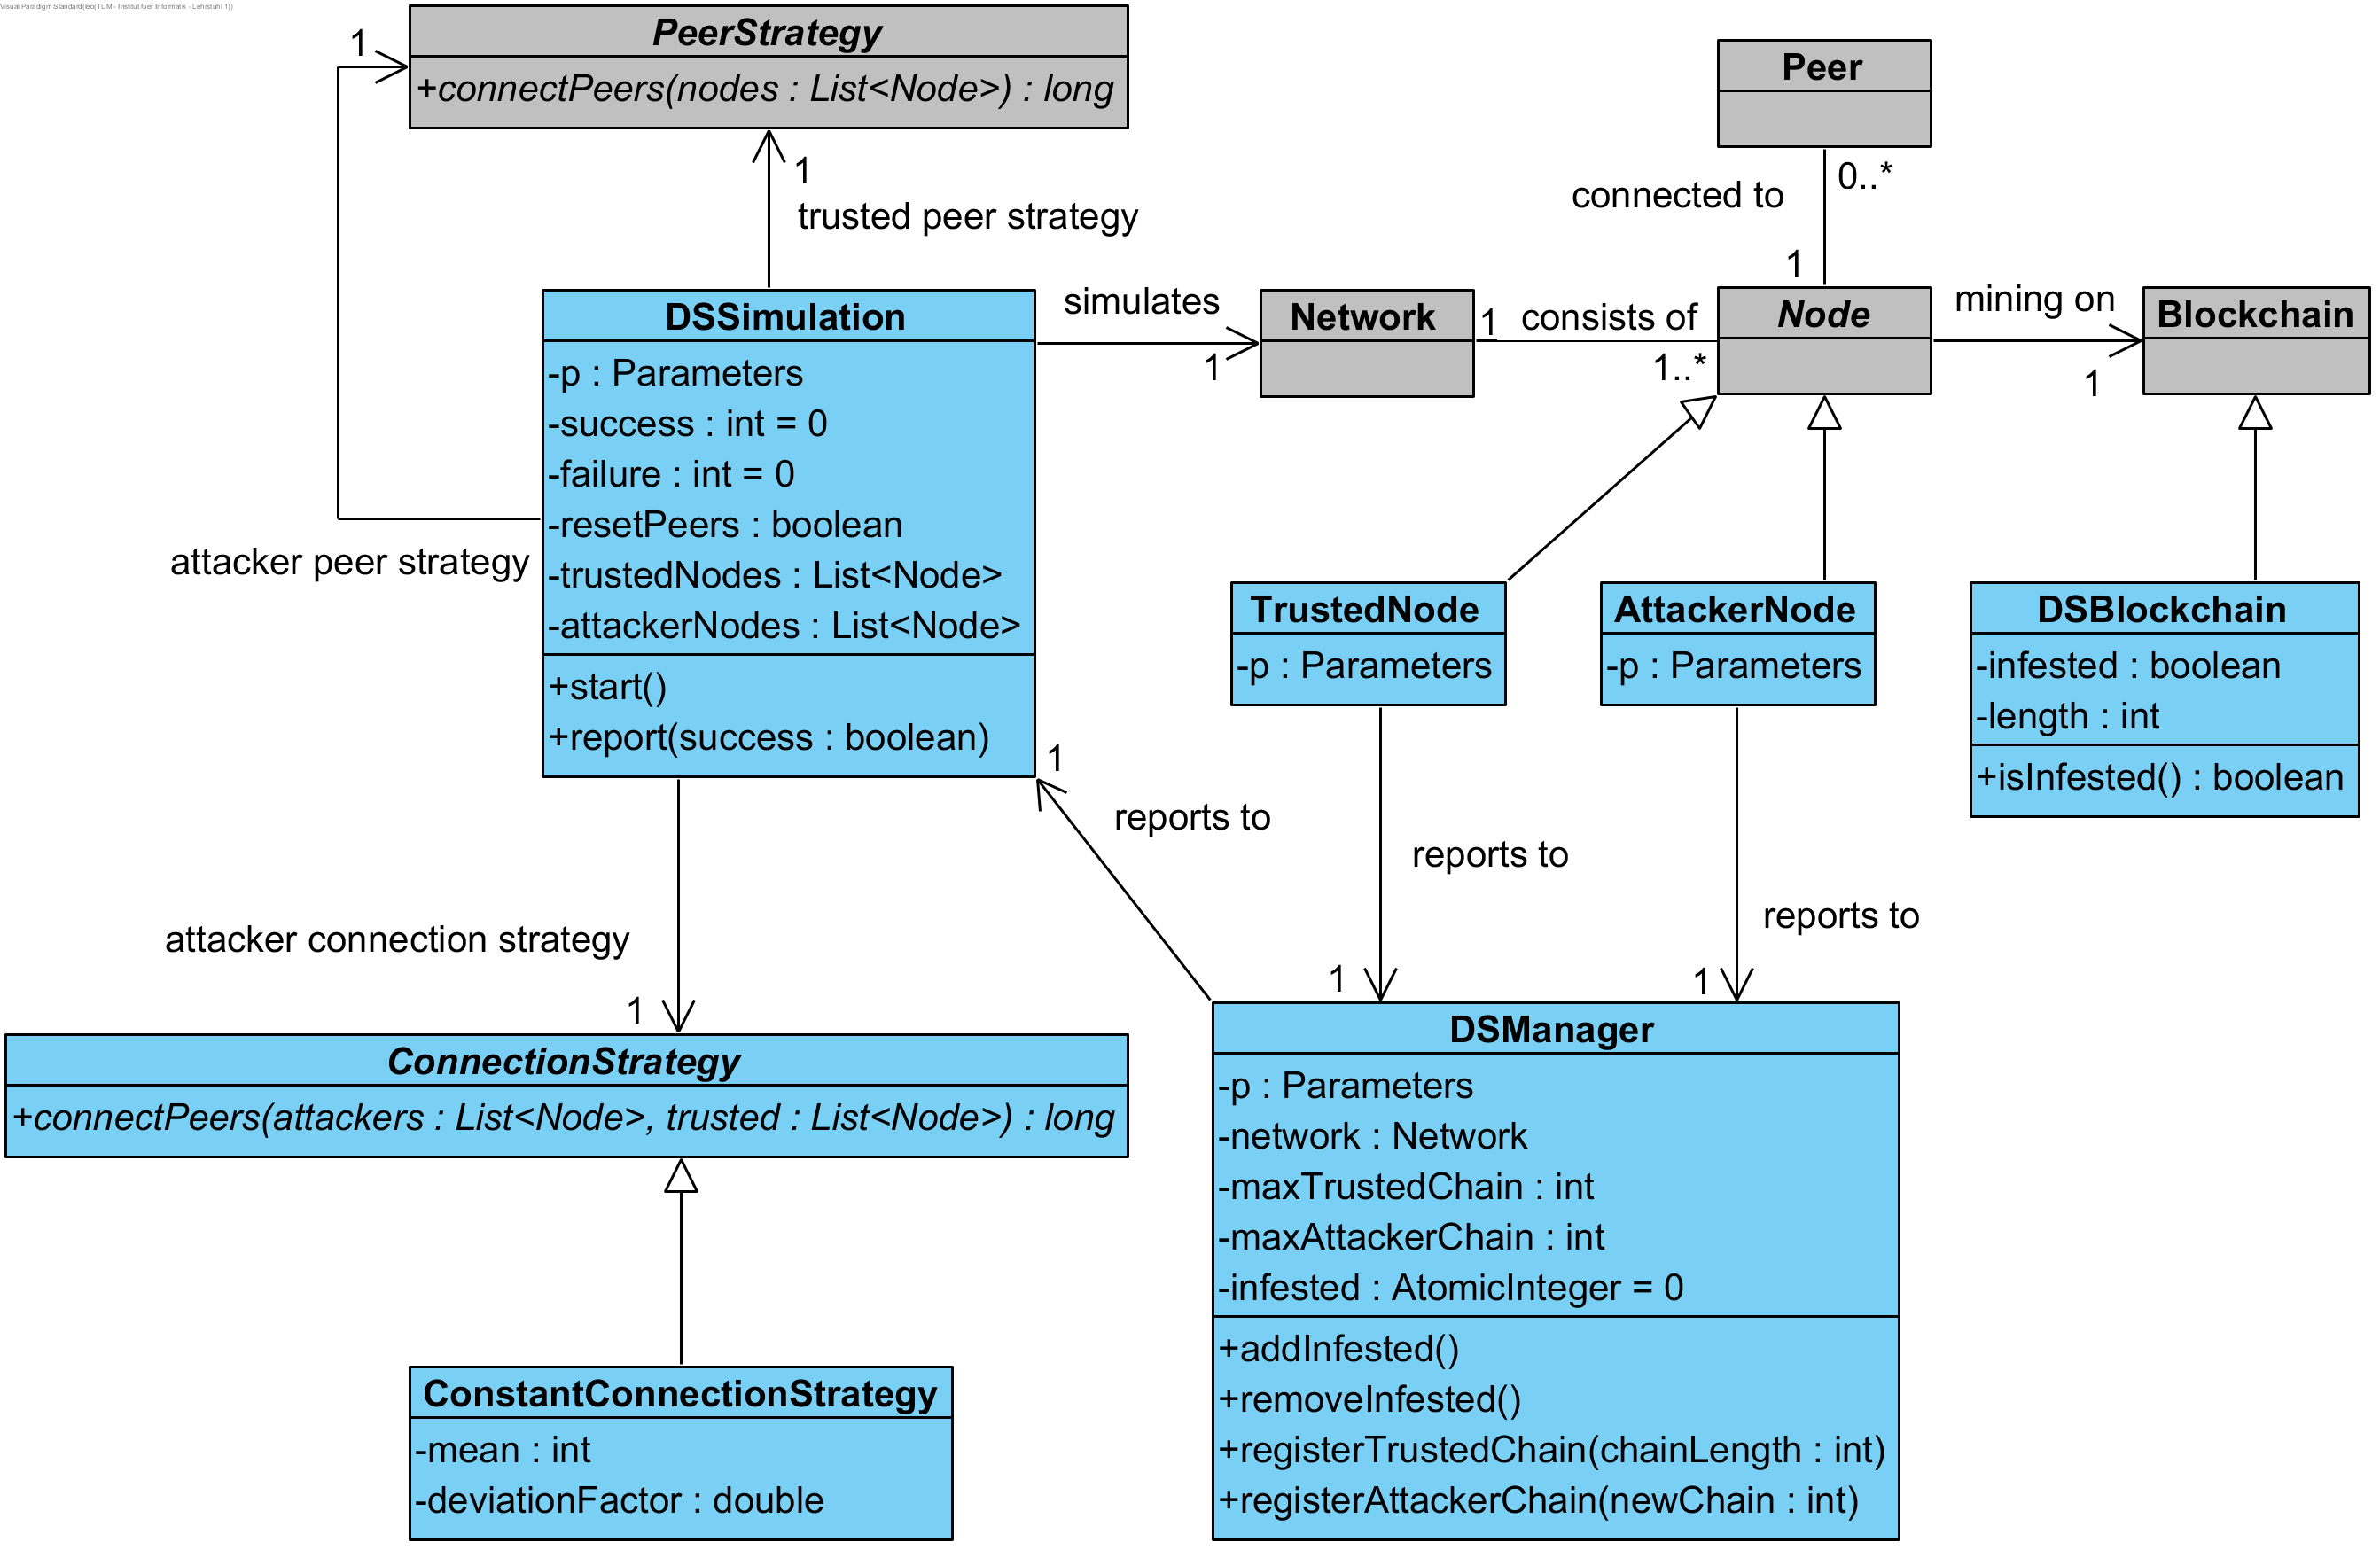
\includegraphics[width=\textwidth]{Simulation.png}
	\caption{Class diagram of the double-spend simulation}
	\label{simulation}
\end{figure}
\subsubsection{DSSimulation}
The DSSimulation initially creates all other instances of this simulation, including the network and its nodes. The class represents the central controller of the simulation, keeping track of successful and failed double-spend attempts and the total number of runs. Once a run is completed, the current attempt is stopped by communicating with the network and the next run is initiated. Parameters and the peer-to-peer graph can be recreated every run, to allow randomization of different simulation aspects. The simulation is generating measures as a result of the number of successful double-spends compared to the total number of runs.
\subsubsection{DSBlockchain}
The blockchain used to simulate double-spend attacks. Instead of modeling entire blocks, the DSBlockchain only consists of a length, which is incremented every time a new block is added. Since double-spend attacks resolve around winning the race between the attackers' and the honest nodes' blockchains, only the number of blocks in the chain are relevant and modeled by our simulation. It is important to note, that despite not explicitly distinguishing between stale and valid blocks by representing the blockchain only by its length, the effects of stale blocks and branches still exist in the network. 

Imagine the current consensus in the network to be a blockchain of length 3. If now two nodes mine a new block at approximately the same time, both send blockchains of length 4 to every peer. In the original protocol, this would result in two different blockchains of length 4 being spread across the network, but using our model, they are indistinguishable. Nevertheless, the nodes of our network simulation still experience one wasted, stale block, as they mined a total of two blocks, but were only able to increase the length of the consented blockchain by one.

To differentiate between blockchains containing the honest payment to the merchant (\textbf{T\textsubscript{M}}) and fraudulent blockchains replacing the payment with a self receiving transaction (\textbf{T\textsubscript{A}}), the DSBlockchain contains a flag indicating whether it is malicious or not.
\subsubsection{DSManager} \label{manager}
A central manager class collecting data sent from every node. By keeping track of the longest attacker and honest blockchains and the amount of nodes mining on a fraudulent chain, the manager determines whether a double-spend attack is successful or if it should be aborted. The attempt of creating a double-spend is considered to be successful, once all nodes are mining on a fraudulent blockchain, after a honest blockchain has been confirmed. This corresponds to the network's consent to be on the double-spending transaction \textbf{T\textsubscript{A}} after the product bought with \textbf{T\textsubscript{M}} has already been shipped (Section \ref{dsa}). 

Since the simulation is potentially running endlessly, if the attacking network never succeeds in passing the honest network's blockchain, the manager considers two parameters in order to decide if the current attempt should be aborted. Firstly, once a maximum lead of the honest network over the attacking network's blockchain is achieved, the success of a double-spend is deemed to be too unlikely and the current run is aborted in failure. Secondly, to avoid the possibility of the honest network maintaining a steady lead, without triggering the first parameter, the simulation is restricted by a maximum length of the blockchains after which the current run fails as well.  The second parameter is especially important, if both networks contain a similar amount of nodes. The nature of these two parameters is further described in Section \ref{faulttolerance}.
\subsubsection{TrustedNode}
This is the implementation of a honest node in the network, working on adding blocks to the longest chain they are currently aware of. The node originally starts working on confirming \textbf{T\textsubscript{M}} with a, by the simulation specified, number of confirmations. After the transaction is confirmed and the product of Section \ref{dsa} has been sent, the node keeps mining on the longest chain. Consequently, it might start mining on the fraudulent blockchain sent by the attacker, as long as it contains more blocks than the original chain. At this point the trusted node is convinced that \textbf{T\textsubscript{A}} is represented in the correct version of the transaction history. However, if the trusted node subsequently receives a longer blockchain containing \textbf{T\textsubscript{M}}, it will switch back to mining on a honest chain. These, infection like, switches are reported to the manager class, until all trusted nodes have been convinced by the attackers or the attempt is aborted.
\subsubsection{AttackerNode}
Contrary to the trusted nodes, the attacking nodes ignore all blockchains not containing the fraudulent transaction \textbf{T\textsubscript{A}} and work exclusively on adding blocks to their private fork. Once \textbf{T\textsubscript{M}} has been confirmed by the trusted network, the attackers start publishing their fraudulent blockchains to convince the network of \textbf{T\textsubscript{A}}.
\subsubsection{ConnectionStrategy} \label{connstrat}
Similar to the framework's PeerStrategy, the ConnectionStrategy adds edges to the network's graph by populating the lists of peers maintained by each node. Instead of creating edges among nodes of a single network, this strategy allows the connection of sets of nodes with each other. Since the network of attacking nodes needs to be able to send its fraudulent blockchains to the honest nodes, this functionality is used to create a connection between both networks. The only strategy currently implemented, connects all attacking nodes with all honest nodes by sampling latency times from the distribution defined in formula \ref{distribution}.
\begin{figure}[ht]
	\centering
  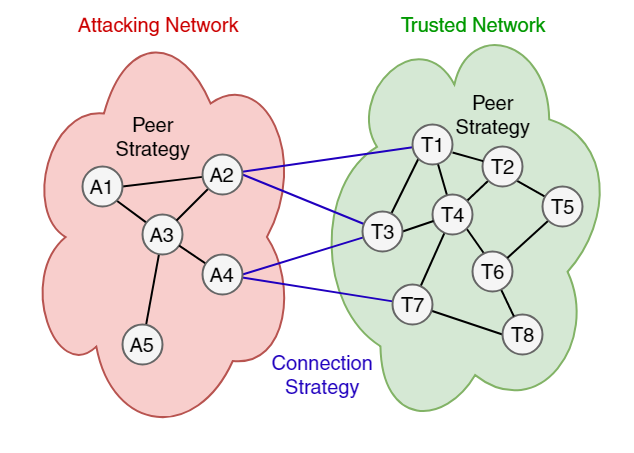
\includegraphics[width=\textwidth]{Network.png}
	\caption{Exemplary simulation network of five attacking and eight trusted nodes}
	\label{network}
\end{figure}

\subsection{Activity Diagram}
A simplified overview of all actions completed by each simulator entity is depicted as an activity diagram in \autoref{activity1}. Note that the \textit{Node} swim lane corresponds to a single trusted or attacking node of the simulation.
\begin{figure}[ht]
	\centering
  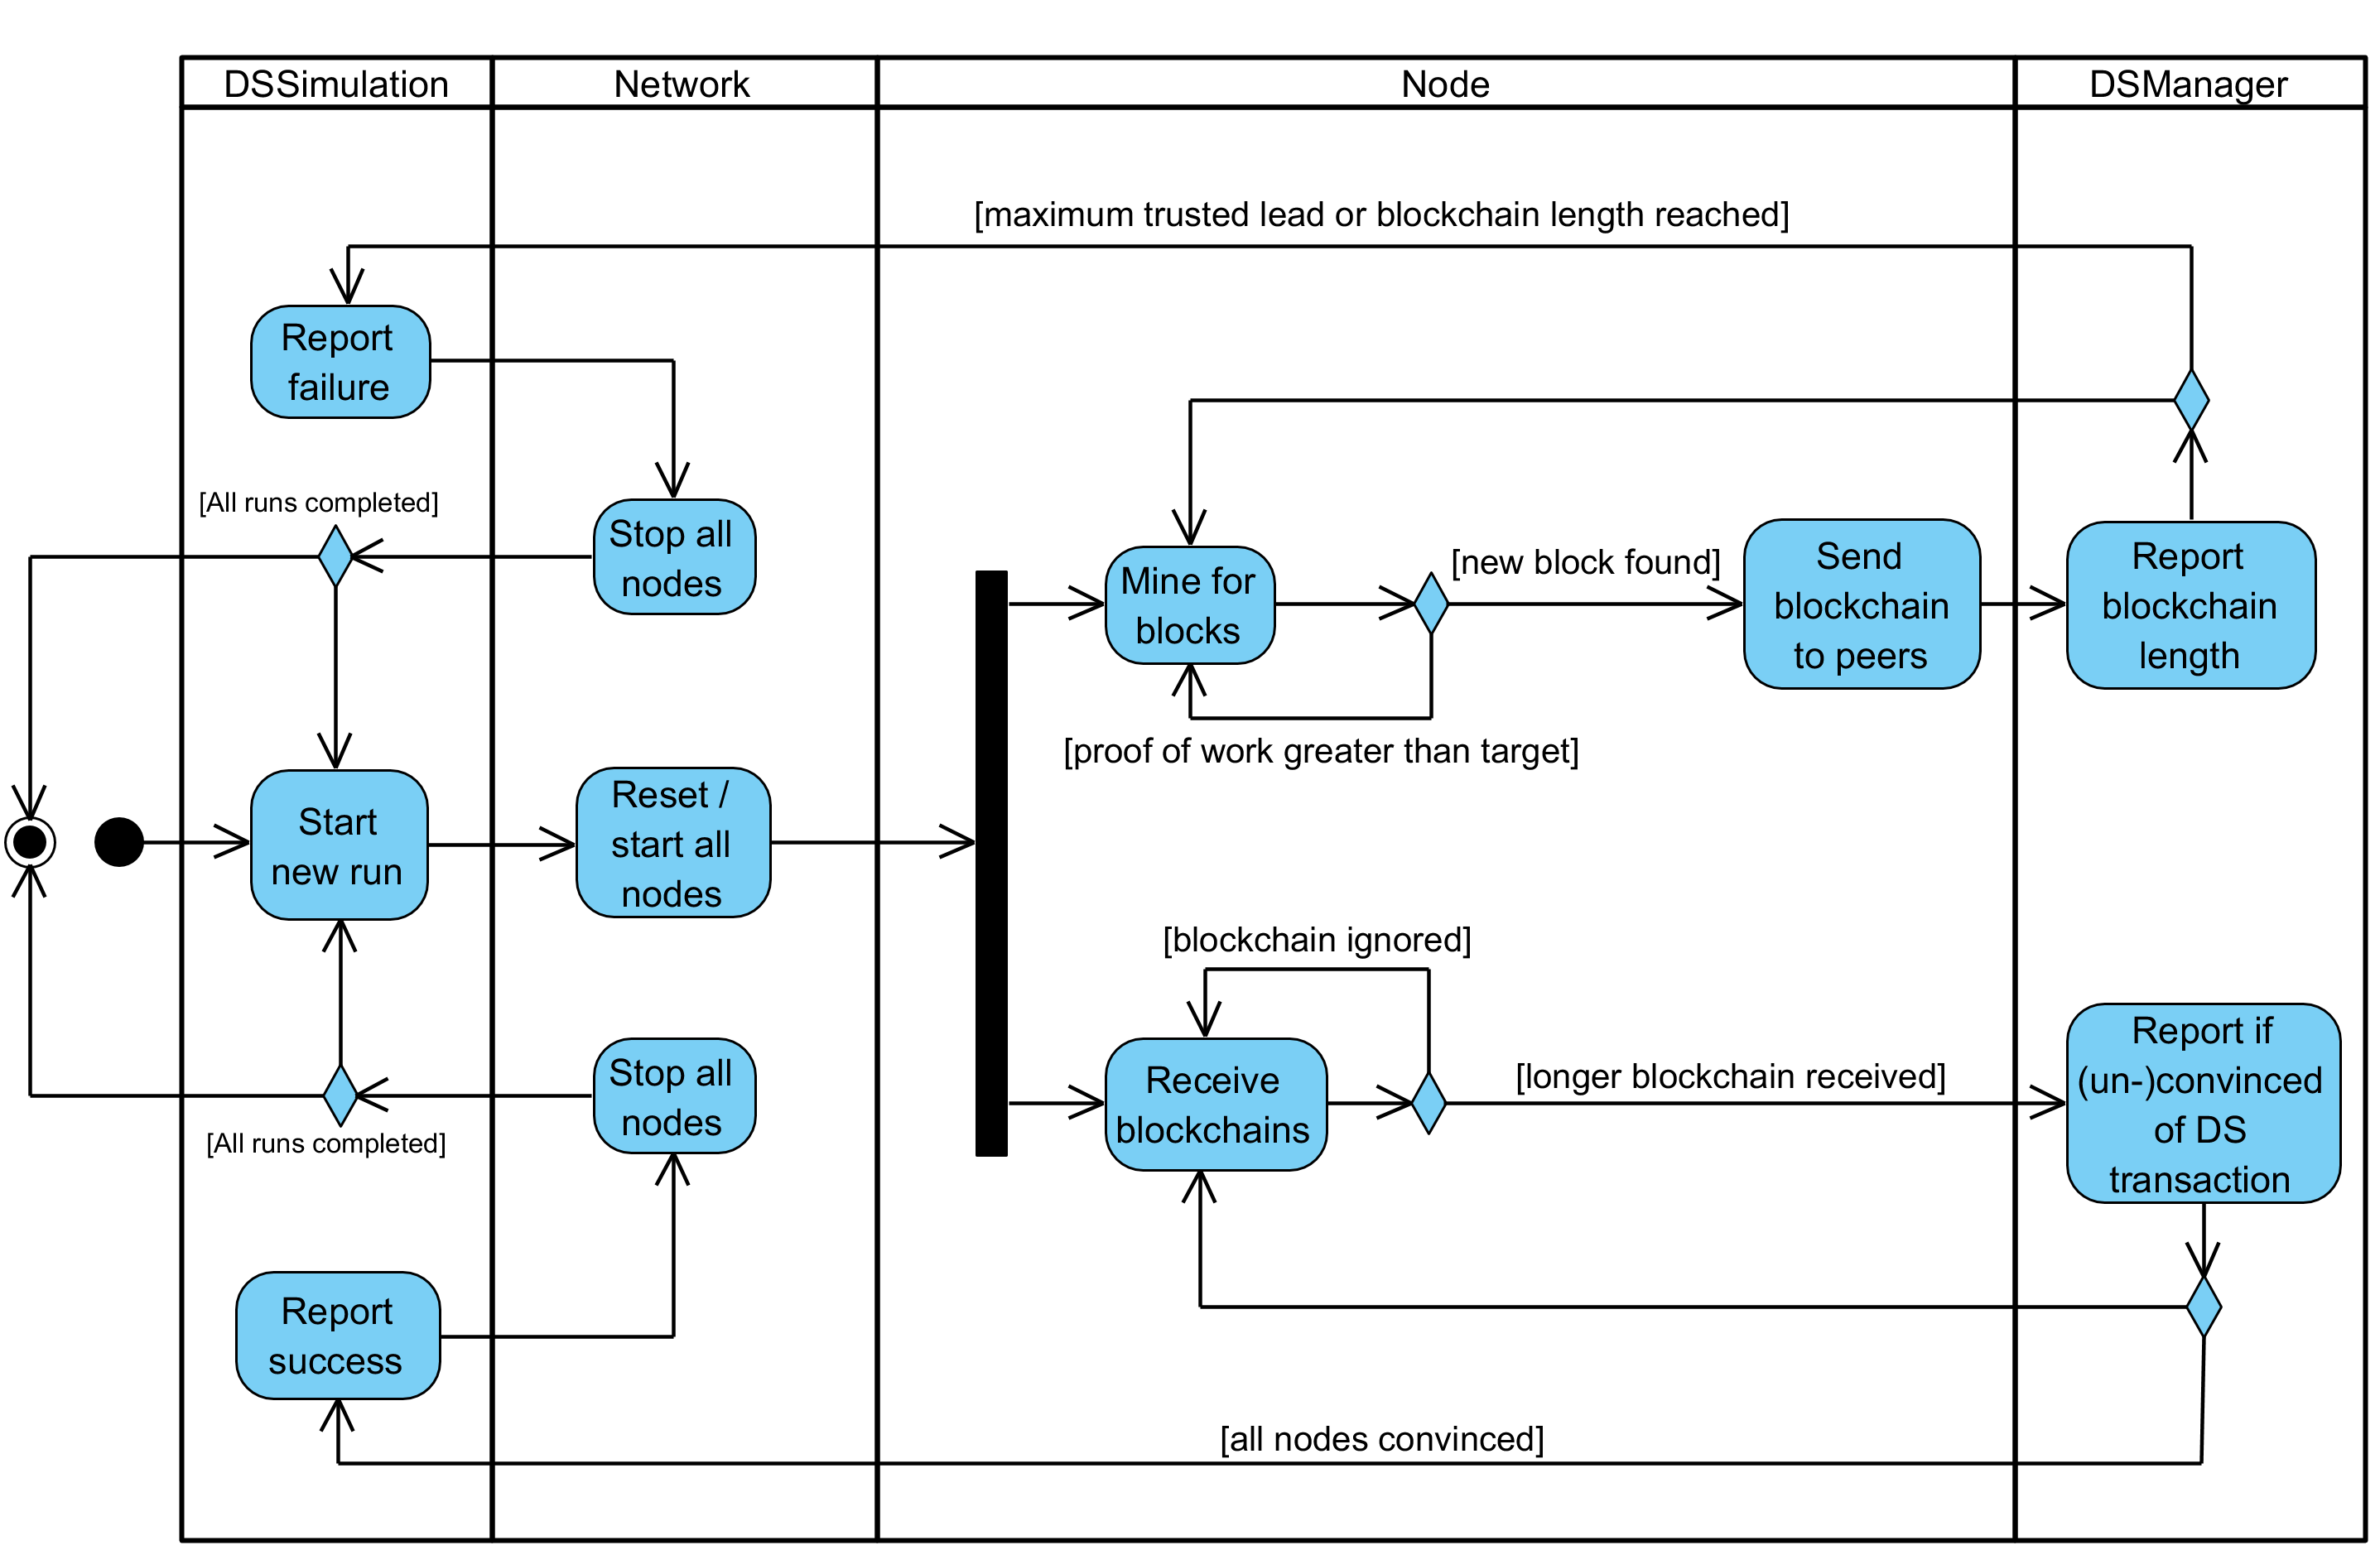
\includegraphics[width=\textwidth]{Activity1.png}
	\caption{Activity diagram of the double-spend simulation}
	\label{activity1}
\end{figure}

\section{Using the Simulator}
The DSSimulation class is the main entry point of the double-spend simulator. It is instantiated by calling the constructor with two peer strategies to create the networks, a connection strategy to connect both networks and a parameters object. If all network strategies have been defined in the parameters object, calling the construct with just the parameters object is sufficient as well. The simulation is started by calling the simulator's \textit{start()} method. After all runs have been completed, the results will be printed out onto the console. 
\subsection{Parameters}
The parameters object is a collection of constants and variables defining the simulated conditions. All parameters can be accessed by their corresponding getter functions.
\subsubsection{Number of Nodes}
The number of nodes consists of the number of attacking and trusted nodes in the networks, consequently there should be at least one node in each of the networks. Since the number of nodes relates to the number of threads created by the simulator, large amounts of nodes should be considered carefully.
\subsubsection{Mining Difficulty Target}
Mining a block in the simulation requires finding a random number $x$ smaller than a target difficulty $t$, whereas $x$ is chosen from an uniform distribution between zero and one (\autoref{uniform}). By defining the target interval as shown in \autoref{tinterval}, the target difficulty precisely represents the probability of the next random number to be a valid proof of work.
\begin{subequations}
\begin{equation}\label{uniform}
x \in X\sim \mathcal{U}(0,1)
\end{equation}
\begin{equation}\label{tinterval}
t \in [0,1]
\end{equation}
\begin{equation}\label{probability}
Pr[X \leq t] = F(t) = t
\end{equation}
\end{subequations}
\subsubsection{Confirmations}
Since it is assumed that \textbf{T\textsubscript{M}} is mined into the first block of the honest blockchain by the trusted network, the number of confirmations represents the number of blocks mined by the trusted network, before the attackers start publishing their secret branch containing \textbf{T\textsubscript{A}}.
\subsubsection{Network Latency Times}
A total of three latency times are defined in the parameters object. These three parameters consist of two latency times for each peer strategy (Section \ref{peerstratsection}) and one for the network connection strategy (Section \ref{connstrat}). The values represent the mean latency times in milliseconds needed to define the Gaussian distribution (Equation \ref{distribution}), in order to sample edge weights of the selected network strategies.
\subsubsection{Network Graph Densities}
When using the random graph strategy (Section \ref{rndgraphstrategy}), the number of edges is defined by the graph density. The parameters object therefore allows specification of a density value for each of the two graphs, in order to simulate 
discrepancies in the quality of attacking and trusted networks. The graph density is a value of the interval $[0,1]$ and represents the ratio of existing edges in a graph compared to the maximum amount of possible edges. Since the created graph has to be connected, the lowest sensible density value is $\frac{2}{n}$, where $n$ is the number of nodes in the network.
\subsubsection{Number of Double-Spend Attempts}
Using the parameters object, the number of simulation runs can be defined. One run consists of a single double-spend attempt on the modeled network, which is either successful or not. By conducting several attempts, a ratio between successful and total attempts can be measured, which is the resulting value of the simulation. This measure is indicative of the trusted network's resistance against double spend attacks.
\subsubsection{Fault Tolerance}\label{faulttolerance}
To avoid the simulation running endlessly, in case the attackers are unable to gain a lead with their secret blockchain fork, it has to be defined when a simulation run can be considered as unsuccessful. This is achieved by the DSManager class using the \textit{maximum lead} and \textit{maximum size} parameters (Section \ref{manager}). Since double spend attacks are theoretically always possible, regardless of the trusted network's lead or the current blockchain length, these two parameters depend on a fault tolerance $\varepsilon$, specified in the parameters object.

Let $t$ and $a$ be the number of trusted and attacking nodes respectively and $t>a$. Using Nakamoto's probability $Q_z$ of an attacker catching up after falling $z$ blocks behind \cite{nakamoto2008bitcoin}, we define $\varepsilon$ as the minimal probability of the attacking network still being able to catch up, before the attempt is considered as unsuccessful. We then derive the maximum value of $z$ that the attackers are allowed to fall behind, in order to maintain the probability $\varepsilon$ of still catching up.
\begin{subequations}
\begin{equation}
Q_z\approx \left( \frac{a}{t} \right) ^{z} < \varepsilon
\end{equation}
\begin{equation}
z < \log_{\frac{a}{t}} \varepsilon
\end{equation}
\begin{equation}
MAX\_LEAD=\begin{cases}
    \infty, & \text{if $a\geq t$}\\
    \ceil{\log_{\frac{a}{t}} \varepsilon}, & \text{otherwise}
  \end{cases}
\end{equation}
\end{subequations}
It can be seen that if $t\leq a$, in this simplified model, the probability of an attacker catching up from a certain deficit is always one. But especially if $t= a$ and a steady lead by the trusted nodes is maintained, our simulation could still be running infinitely. Therefore, the simulation will stop in failure, after a maximum blockchain length (Equation \ref{maxlength}) is reached. 
\begin{equation}\label{maxlength}
MAX\_LENGTH= \frac{1}{100\varepsilon}
\end{equation}

\subsection{ParametersBuilder}
The parameters object can be created using a ParametersBuilder, which is offering setter functions to all available parameters. The ParametersBuilder is an implementation of the builder pattern and can be used to instantiate the parameters object as shown in \autoref{builderlist}. Undefined parameters will be set to the default values listed in \autoref{prop}.
\begin{lstlisting}[language=Java, caption=Initializing parameters using the ParametersBuilder,label=builderlist]
ParametersBuilder b = new ParametersBuilder();
Parameters p1 = b.setTrustedNodes(40)
	.setAttackerNodes(13)
	.setAttackerPeerStrategy(PeerStrategyEnum.CONSTANT)
	.setTrustedLatency(500)
	.setConfirmations(6)
	.build();
Parameters p2 = b.setAttackerNodes(18)
	.build();
\end{lstlisting}
\subsubsection{Randomized Parameters}
The simulator and the parameters object support randomization of the confirmation, latency and density parameters. If parameters are randomized, a new value will be generated according to the specified bounds, after every new simulation run. The parameters can be randomized by providing the selected lower and upper bounds to the ParametersBuilder, before building the parameters object. Parameters can be reset to specific values, by calling the builder's setter function and rebuilding the object.
\begin{lstlisting}[language=Java, caption=Randomizing parameters using the ParametersBuilder]
ParametersBuilder b = new ParametersBuilder();
Parameters p = b.randomizeConfirmations(1, 10)
                .randomizeAttackerLatency(10, 50)
                .randomizeAttackerGraphDensity(0.2, 0.7)
                .build();
\end{lstlisting}
\subsubsection{Loading from Property Files}
Using the ParametersBuilder, parameters can be loaded from external property files, by providing the corresponding file name as shown in \autoref{proplist}. A full description of the property file's structure and usage can be found in \autoref{prop}.

\begin{lstlisting}[language=Java, caption=Loading parameters from property file,label=proplist]
ParametersBuilder b = new ParametersBuilder()
Parameters p;
try {
	p = b.loadFromProperty("parameters.txt")
	     .build();
} catch (IOException ex) {
	System.err.printf("Error: %s\n", ex);
	System.exit(1);
}
\end{lstlisting}
\subsection{The Compiled Simulator}
After compilation, the uploaded simulator in \cite{github} can be controlled by providing a property file containing the selected parameter configuration as a command line argument.
\begin{lstlisting}[caption=Launching the simulator from the command line,label=cmd]
java -jar Blockchain.jar "parameters.txt"
\end{lstlisting}
%------- chapter 5 -------

\chapter{Evaluation}

\section{Design}
	
\section{Objectives}

\section{Results}

\section{Findings}

\section{Discussion}

\section{Limitations}
\begin{itemize}
\item Scheduling
\item All attacking Nodes have equal, constant latency to each trusted node
\item Network creation not perfectly random

\end{itemize}

%------- chapter 6 -------

\chapter{Model}


%------- chapter 7 -------

\chapter{Summary}

\section{Status}

\subsection{Realized Goals}

\subsection{Open Goals}
\begin{itemize}
\item All attacking Nodes have equal, constant latency to each trusted node
\item Network creation not perfectly random
\end{itemize}
\section{Conclusion}

\section{Future Work}
\begin{itemize}
\item validate models mentioned in related work
\item implement other attacks mentioned in related work on blockchains using framework
\item identify missing parameters
\item conduct more tests
\item using result: economics of dsa?
\end{itemize}




\appendix

\chapter{Property Files} \label{prop}
Property files can be used to permanently store parameters and allow simple configuration of the simulated conditions. The property file's structure is a list of key-value pairs, defined as an assignment of values to parameter names (keys) as shown in \autoref{propstruc}. In the following a short summary of all available parameters and possible values will be presented.
\begin{lstlisting}[caption=Property file structure,label=propstruc]
<parameter1> = <value1>
<parameter2> = <value2>
...
\end{lstlisting}
\subsubsection{NUM\_TRUSTED, NUM\_ATTACKER}
The number of honest and attacking miners in the simulated network should be greater than zero. Since each node corresponds to an additional program thread, higher numbers of nodes should be considered carefully.
\subsubsection{DIFFICULTY}
The difficulty target of mining a block. Should be specified as a floating point number between 0 and 1.
\subsubsection{CONFIRMATIONS}
The number of blocks needed to confirm a transaction should be non-negative.
\subsubsection{LAT\_TRUSTED, LAT\_ATTACKER}
The mean latency in milliseconds used to create the Gaussian distribution presented in Section \ref{distribution} should be non-negative. Parameters for trusted and attacking networks can be defined individually to allow simulation of different connection qualities in the networks.
\subsubsection{LAT\_CONNECTION}
The mean latency in milliseconds used to model the connection between attacking and trusted network.
\subsubsection{DENS\_TRUSTED, DENS\_ATTACKER}
The graph density of the attacking and trusted networks as defined by the \hyperref[rndgraphstrategy]{RndGraphStrategy}. Since the created graph has to be connected, the specified floating point value should be in the range of $[\frac{2}{n}, 1]$, where $n$ is the number of nodes in the graph.
\subsubsection{RUNS}
The number of double-spend attempts carried out by the Simulator for each simulation.
\subsubsection{EPSILON}
The fault tolerance corresponding to Section \ref{faulttolerance} should be a floating point value in the range of $(0, 1)$.
\subsubsection{LOGGING}
Controls the amount of console output. Possible values are \textit{INFO}, \textit{FINE}, \textit{FINER}, \textit{FINEST}, whereas the amount of detail corresponds to $\textit{INFO} < \textit{FINE} < \textit{FINER} < \textit{FINEST}$.
\subsubsection{T\_PEER\_STRAT, A\_PEER\_STRAT}
These parameters can be set to select the peer strategies used to create the networks. Strategies requiring the definition of an adjacency matrix cannot be specified using property files. Possible values are therefore: \textit{CONSTANT}, \textit{EUCLIDEAN}, \textit{RANDOM}, referring to the strategies defined in Section \ref{peerstratsection}.
\subsubsection{CONN\_STRAT}
This parameter can be set to select the connection strategies used to create a link between attacking and trusted network. Currently the only possible value is \textit{CONSTANT}.
\subsubsection{Randomized Parameters}
Bounds of randomized parameters can be specified by providing lower and upper bounds, where $lower < upper$ (\autoref{boundstruc}). If bounds of a parameter have been specified by the loaded property file, the parameter will automatically be randomized during the simulation. Randomizable parameters are latencies, graph densities and the number of confirmations.
\begin{lstlisting}[caption=Defining bounds of randomized parameters,label=boundstruc]
<parameter1_BOUNDS> = <lower1>, <upper1>
<parameter2_BOUNDS> = <lower2>, <upper2>
...
\end{lstlisting}
\subsubsection{Default Values}\label{defaultval}
Undefined parameters will be initialised with default values as defined in \autoref{default}. 
\begin{lstlisting}[caption=Default parameter values,label=default]
NUM_TRUSTED    = 32
NUM_ATTACKER   = 16
DIFFICULTY     = 0.00001
CONFIRMATIONS  = 6
LAT_TRUSTED    = 10
LAT_ATTACKER   = 10
LAT_CONNECTION = 10
DENS_TRUSTED   = 0.8
DENS_ATTACKER  = 0.8
RUNS           = 100
EPSILON        = 0.00001
LOGGING        = FINE
T_PEER_STRAT   = RANDOM
A_PEER_STRAT   = RANDOM
CONN_STRAT     = CONSTANT
\end{lstlisting}
\clearpage

\listoffigures
\clearpage

\listoftables
\clearpage

\bibliography{thesis}
\bibliographystyle{alpha}

\end{document}
